%!TEX root = ../dissertation.tex

\hypertarget{(chap:capitolo3)}{}
\chapter{Sistemi di raccomandazione}
In questo capitolo vedremo un riassunto della teoria riguardante i sistemi di raccomandazione, dei suoi diversi approcci e degli algoritmi presenti nella tesi.
\section{Introduzione}
Uno dei campi più popolari al momento verso cui si rivolge una particolare attenzione è quello dei \bit{sistemi di raccomandazione}{overview_rs} (RS), in quanto l'attività online sta aumentando sempre più e nascono sempre più spesso nuovi servizi che permettono di scegliere oggetti, siano questi prodotti, video, musica, film o molto altro, da cataloghi vastissimi. I sistemi di raccomandazione permettono di navigare questi cataloghi andando a cercare gli oggetti che risultino più interessanti per l'utente.

\section{Preliminari}
In generale possiamo dire che un RS si compone di diversi elementi, in primo luogo abbiamo i cosidetti 'attori' del problema, gli user e gli item, rispettivamente gli utenti del sistema (U) e gli oggetti che si vuole consigliare (I). Abbiamo a disposizione inoltre informazioni riguardo l'interazione tra user e item solitamente sotto forma di feedback implicito o esplicito, questa misura viene definita rating. Questi vengono utilizzati dal RS, insieme con eventuali dati legati al contesto di user e item, per effettuare raccomandazioni.

\subsection{Feedback impliciti / espliciti}
Solitamente le informazioni che legano user e item, ossia i rating, possono essere di due tipi:
\begin{itemize}
	\item Implicito: 1 se c'è stata interazione tra lo user e l'item, 0 se non c'è stata;
	\item Esplicito: valutazione numerica nell'intervallo $[1,scale]$, 0 se non c'è stata interazione.
\end{itemize}

Nel nostro caso di studio però ci ritroviamo a metà strada in quanto, se per esempio considerassimo la quantità come un dato esplicito ci troveremmo così ad avere un dato su una scala non continua, mentre se lo facessimo come se fosse implicito trascureremmo delle informazioni che possono in qualche modo fornire una misura di interesse.

\subsection{User-item interaction matrix}
\begin{minipage}[H]{0.45\textwidth}
	\begin{center}
		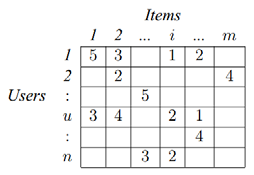
\includegraphics[width=5.5cm]{figures/Sample-of-user-item-matrix}
		\captionof{figure}{Esempio user-item\\ interaction matrix esplicita.}
		\label{tab:user_item_matrix}
	\end{center}
\end{minipage}
\begin{minipage}[H]{0.55\textwidth}
	I rating sono organizzati in matrici, dette user-item interaction matrix o semplicemente matrici dei rating (R), dove sulle righe abbiamo gli utenti mentre sulle colonne abbiamo gli oggetti, nell'incrocio abbiamo riportato il rating. 
	La matrice come detto può essere implicita o esplicita e le celle vuote corrispondono allo 0.
	Quando scriviamo $r_{ui}$ intendiamo che $u$ è lo user e $i$ è l'item.
\end{minipage}

\subsection{Obiettivo}
L'obiettivo del sistema può essere quello di consigliare ad uno user una lista di N item, detta \glo{TopN} che si ritiene possano interessargli, oppure dato un item si può trovare una lista di item che si considerino simili allo stesso in acccordo con i 'gusti' dello user.

\section{Approcci}
Definito quindi il task abbiamo diversi modi per poter soddisfare il nostro obiettivo, in generale abbiamo due principali categorie di RS:
\begin{itemize}
	\item \textbf{Non Personalizzato}: andiamo a consigliare i prodotti che globalmente risultano più popolari, ossia che abbiano complessivamente ricevuto più valutazioni, o quelli con rating più alto. Questo approccio non va a considerare le informazioni relative il singolo user;
	\item \textbf{Personalizzato}: ci sono diversi approcci che vedremo nelle sezioni successive, in generale si fanno raccomandazioni basate sulla similarità tra user. I due approcci più famosi sono il collaborative filtering, dove si cerca di consigliare item ad uno user basandosi su user simili, e il content-based filtering si cerca di raccomandare item simili a quelli con cui si ha già interagito.
\end{itemize}

Nelle sezione successive andiamo a spiegare più nel dettaglio il collaborative e conte-based filtering.

\subsection{Collaborative filtering}
Il \bit{collaborative filtering}{CF} è un approccio agli RS basato sulla similarità, raccomandiamo ad uno user item interessanti per altri user simili ad esso, e viceversa item simili ad altri item per cui ha dimostrato interesse.
La similarità può essere quindi di due tipi: item-based, basata quindi sulla similarità tra prodotti o user-based ossia su quella tra user.
Ci sono due approcci possibili al collaborative filtering:
\begin{itemize}
	\item Memory-based: utilizziamo la matrice dei rating per calcolare la similarità tra user e item, metodi basati sull'algoritmo K nearest neighbour;
	\item Model-based: utilizziamo dei modelli che attraverso degli algoritmi permettono di predire il rating su item non valutati.
\end{itemize}

\subsubsection{User k-nearest neighbour}
User k-nearest neighbour (UserKnn) è un metodo memory-based che fa uso della matrice dei rating, ogni user avrà quindi un proprio 'profilo', ossia la propria riga nella matrice dei rating. 
Per esempio immaginiamo di avere dei rating impliciti, l'idea è quella di calcolare la similarità tra tutti gli user, ad esempio tra due user $u$ e $v$ questa sarà calcolata con la funzione coseno $s_{uv} = \frac{|I_{u} \cap I_{v}|}{\sqrt{|I_{u}||I_{v}|}}$, dove $I_u$ sono gli item valutati dallo user $u$. Dopo questa operazione è possibile calcolare il rating previsto per ogni item $i$ non valutato rispetto ad uno user $u$ con la seguente formula $\hat{r_{ui}} = \frac{1}{k} \sum_{v\in N_{i}^k(u)} s_{uv}$, dove $N_{i}^k(u)$ è la lista dei k user, che hanno valutato l'item $i$, più simili allo user $u$.\\
Più in generale selezioniamo i k user con similarità più alta con il nostro user target e calcoliamo la media pesata dei loro rating usando come pesi la similarità.\\
Fatto questo si procede ad ordinare per ciascuno user tutti i prodotti secondo i rating ottenuti e si ottiene così la lista $TopN$ degli item più interessanti.\\
Questo metodo funziona senza informazioni relative alle caratteristiche degli user o item e può gestire rating espliciti o impliciti con formule leggermente diverse.

\subsubsection{Item k-nearest neighbour}
Item k-nearest neighbour (ItemKnn) è un metodo memory-based molto simile al precedente, qui si va a considerare però gli item da raccomandare e il loro profilo è la propria colonna della rating matrix. Si calcola la similarità tra tutti gli item e dato uno user si procede a calcolare il rating stimato sugli item che non ha valutato, trovando per ciascuno di essi la lista di K item più simili ad esso, poi calcola la media pesata dei rating dei K item selezionati usando come peso la similarità. Le formule sono molto simili alle precedenti solo che al posto di usare il profilo dello user si usa quello dell'item.
 
\subsubsection{Matrix Factorization}
Nell'approccio model-based, Matrix Factorization (MF) è uno dei modelli più famosi, questo si basa sul concetto che si possa mappare user e item verso uno spazio delle feature comune di una certa dimensionalità k. Creiamo quindi due matrici P e Q, dove P è una matrice avente sulle righe gli user e come colonne le k feature, mentre Q è una matrice avente sulle righe le k feature e sulle colonne gli item. Vogliamo ottenre una approssimazione della rating matrix attraverso la moltiplicazione di P e Q, ossia $R \approx P \cdot Q^{T} = \hat{R}$, come nella Figura \ref{tab:MF}.\\
\begin{center}
	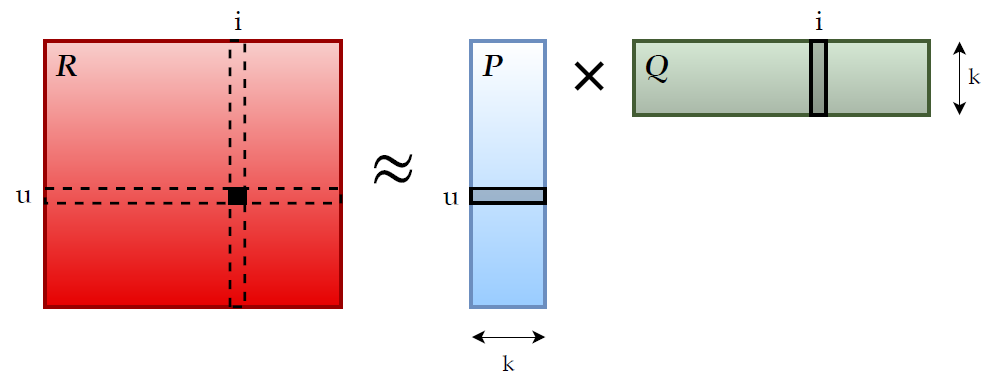
\includegraphics[width=14.5cm]{figures/MF_disegno}
	\captionof{figure}{Rappresentazione visiva delle matrici R, P e Q.}
	\label{tab:MF}
\end{center}
Quello che otteniamo è quindi un profilo sia per gli user che per gli item rispetto lo stesso spazio delle feature. Il problema maggiore risulta però essere quello di ottenere queste due matrici, possiamo farlo definendo la seguente funzione di loss $L(P,Q) = min_{P,Q} \left\lVert R - PQ^T\right\rVert^2 +\lambda(\left\lVert P \right\rVert^2 + \left\lVert Q \right\rVert^2)$. Alleniamo il modello fissando in modo alternato le matrici P e Q, cercando quindi di ridurre dopo ciascuna iterazione la differenza tra $R$ e $PQ^T$, la $\lambda$ è un hyper-paramentro utile per la regolarizzazione, infatti permette di penalizzare in base alla norma delle matrici P e Q, facendo sì che queste abbiano una norma vicina allo zero.\\
Una volta che il modello è allenato possiamo predire il rating dato da uno user $u$ su un item $i$ moltiplicando i profili corrispondenti $\hat{r}_{ui} = P_u \cdot Q_{i}^{T}$.

\subsubsection{Variational Auto-Encoder for CF (VAECF)}
Il VAECF è un \bit{Variational Auto-Encoder}{Kingma_2019} (VAE) che si basa sull'\bit{Auto-Encoder}{bank2021autoencoders} (AE), una rete neurale composta da due parti: l'encoder (E) e il decoder (D).
L'encoder si occupa di ridurre la dimensionalità della distribuzione iniziale, ottenendo quindi una sua rappresentazione nello spazio latente. Il decoder prende questa rappresentazione e cerca di ricostruire la distribuzione iniziale, possiamo dire che, data una distribuzione $x$, l'obiettivo sia quello di far sì che $x \approx D(E(x)$.
L'AE usando questa funzione obiettivo è però molto soggetto all'overfitting, ciò che invece vorremmo è una spazio latente regolarizzato da cui poter generare nuove distribuzioni.
Il VAE è infatti un modello generativo che apprendere le distribuzioni iniziali e le mappa verso una rappresentazione nello spazio latente, ciò che si vuole fare è regolarizzare questo spazio in modo da poter generare da questo nuove distribuzioni. Nel VAE l'encoder mappa la distribuzione iniziale $x$ verso due valori $(\sigma_x, \mu_x)$, media e varianza di una distribuzione gaussiana $N(\sigma_x, \mu_x)$, da questa poi si estrae un sample $z$ e attraverso il decoder si cerca di ricondurlo alla distribuzione iniziale $x$. Possiamo vedere queste operazione nella Figura \ref{tab:VAE_dis}. 
\begin{center}
	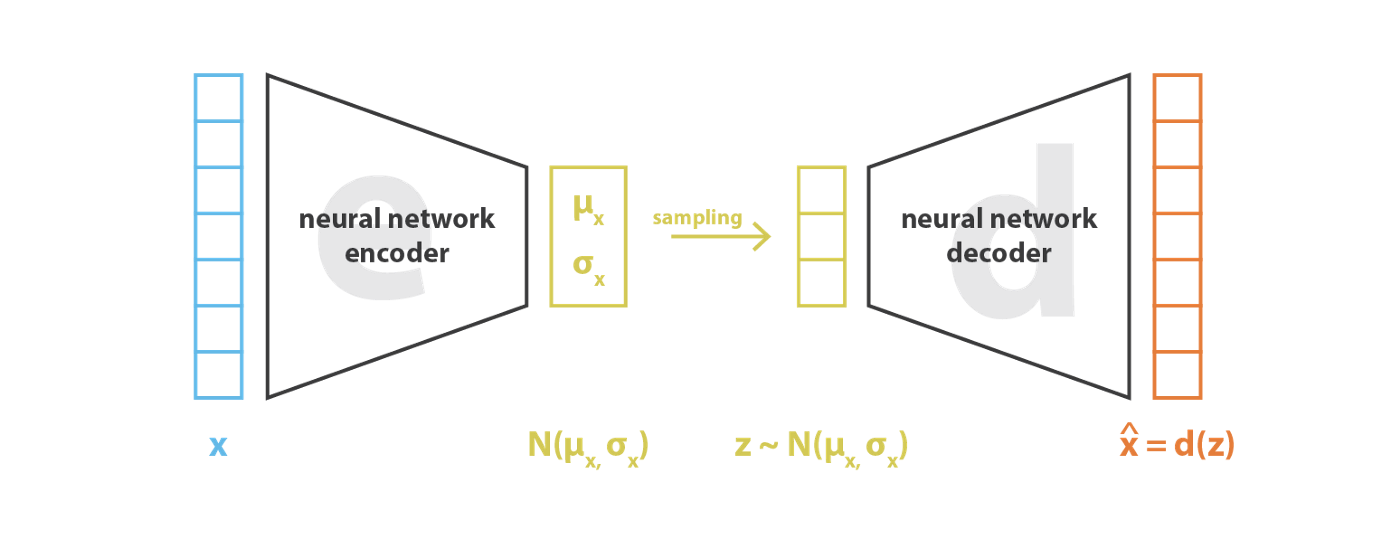
\includegraphics[width=14.5cm]{figures/VAECF.png}
	\captionof{figure}{Rappresentazione grafica del VAE.}
	\label{tab:VAE_dis}
\end{center}
Per permettere di usare l'algoritmo \glo{backpropagation} si esegue il sampling da una distribuzione $N(0,1)$ e poi si riscala $z$ rispetto quella data dalla rappresentazione $N(\sigma_x, \mu_x)$, questo passaggio viene chiamato 'reparametrisation trick'.\\
La funzione obiettivo è definita come segue:
$$L(x) = \left\lVert x - D(z) \right\rVert^2 + KL[N(\sigma_x, \mu_x),N(0,1)]$$
Si nota il trade-off tra funzione obiettivo dell'AE e la regolarizzazione attuata sulla rappresentazione delle distribuzioni interne grazie alla KL divergence, una funzione che misura la distanza tra la distribuzione $N(\sigma_x, \mu_x)$ e $N(0,1)$, cercando di ridurla il più possibile.
Rispetto ai modelli precedenti che potevano funzionare sia con rating espliciti che impliciti, il VAECF accetta solo quest'ultimi. Il modello prende in input la matrice dei rating impliciti andando a considerare ogni riga come una distribuzione associata allo user e per ciascuno di essi ritorna la distribuzione generata da cui poi si possono estratte gli item consigliati andando a selezionare quelli che riportano valori più alti nella distribuzione data dal decoder.

\subsection{Content-based filtering}
Il \bit{content-based filtering}{content_based} è un approccio che si basa sull'idea di consigliare item simili a quelli con cui si è già interagito.\\
Ciascun item possiede delle feature, per esempio nel caso si abbia come item dei film queste potrebbero essere i generi, l'insieme delle feature può essere mappata su di un vettore delle feature, per ogni item quindi si riporta nel vettore 1 se possiede quella feature, 0 altrimenti, questo permette di definire un profilo per l'item.
Una volta fatto ciò si procede a creare anche un profilo per lo user, ci sono diversi modi per farlo ma per esempio si può considerare tutti i profili degli item con cui si è interagito e farne quindi la media pesata basata sui rating corrispondenti.
Ottenuto un profilo anche per lo user si può calcolare la similarità tra di esso e quello degli item per poi ordinarli secondo similarità ottenendo così la lista $TopN$.

\section{Valutazione}
Quanto abbiamo visto finora sono metodi che ci permettono di effettuare le raccomandazioni, vogliamo trovare però anche il modo per poterle valutare. Per prima cosa dobbiamo dividere le matrici dei rating in training e test set.\\
Per fare ciò andiamo ad eseguire uno shuffle delle coppie (user, item) e si va ad assegnare al training set l'80\% delle coppie e le restanti al test set, questo sistema non ci assicura che uno user sia presente nel training set.
Date le raccomandazioni fornite dal RS vogliamo valutarle rispetto due aspetti principali: il rating e il ranking.
Il primo aspetto riguarda semplicemente la diversità tra i rating stimati da quelli reali delle coppie (user, item) del test set, queste metriche non vengono solitamente usate in quanto non è un buon modo per valutare un RS perché non ci permette di capire se un'item consigliato sia rilevante.
Andando invece a considerare il concetto di ranking ci rendiamo conto che sia più legato a ciò che vogliamo andare a valutare, le metriche annesse considerano rilevanti gli item presenti nel test set e vanno a verificarne la posizione nella lista $TopN$.
In generale le metriche si applicano a ciascuno user e il risultato finale è la media dei singoli risultati.

\subsection{AUC}
L'\bit{AUC}{dhanjal2015auc} (Area Under the Curve) è una metrica che permette di valutare un RS basandosi sul numero di coppie di item rivelanti e non presenti nella $TopN$, dove un item non rilevante ha uno score minore rispetto a quello di uno rilevante. Questa metrica assegna lo stesso peso a ciascun item rispetto il ranking, questo significa che non controlla la posizione in cui si trovano gli item più interessanti. Vediamo di seguito la formula:
$$AUC = \frac{1}{|N^{+}|\cdot|N^{-}|}\sum_{i \in N^{+}} \sum_{j \in N^{-}} [s(i) > s(j)]$$
Il termine $N^{+}$ è l'insieme degli item presenti nel test set, mentre $N^{-}$ sono tutti gli item rimanenti. $s(i)$ è la valutazione data dal RS sull'item $i$, quello che si fa è andare a contare il numero di coppie di item in ordine nella $TopN$ andando a vedere gli score assegnati loro.
Utilizziamo la funzione $[s(i) > s(j)]$ che restituisce 1 se lo score dell'item rilevante è maggiore, 0 altrimenti. Infine dividiamo il numero di coppie ordinate in modo correto per il numero di coppie totali.\\
Il valore dell'$AUC \in [0,1]$, dove più il valore si avvicina ad 1, minori saranno le coppie in ordine sbagliato.

\subsection{nDCG@k}
La metrica \bit{nDCG@k}{wang2013theoretical} (normalized Discount Cumulative Gain) ci permette di calcolare una misura basata sulla posizione degli item rilevanti, ossia quelli del test set, tra i primi k item della lista $TopN$.

\begin{minipage}[H]{0.5\textwidth}
	$$DCG@k = \sum_{i=1}^{k} \frac{2^{rel_i} - 1}{log_{2} (i + 1)}$$
\end{minipage}
\begin{minipage}[H]{0.5\textwidth}
	$$IDCG@k = \sum_{i=1}^{|REL_i|} \frac{2^{rel_i} - 1}{log_{2} (i + 1)}$$
\end{minipage}
\newline

Ed infine per cacolare la $nDCG@k$ usiamo la seguente formula:
$$nDCG@k = \frac{DCG@k}{IDCG@k}$$

Per prima cosa dobbiamo dire che la metrica lavora su una parte della lista $TopN$, ossia la parte contentente i primi K item che definiamo come $TopK$.\\
Gli item più rilevanti nel nostro caso sono gli item presenti nel test set.\\
Andiamo ora ad analizzare numeratore e denomicatore per capire meglio la loro funzione.
\begin{itemize}
	\item La $DCG@k$ si basa sull'idea che gli item più rilevanti debbano trovarsi il più possibile in testa alla lista $TopK$, quindi si vuole penalizzare un item sempre di più via via questo si trovi nella coda della lista, per far ciò il denominatore aumenta all'aumentare della posizione seguendo una scala logaritmica. 
	\item La $IDCG@k$ è equivalente a calcolare la $DCG@k$ sulla lista $TopK$ ideale, ossia la lista riportante tutti gli item ordinati in modo ideale secondo score nella posizione corretta, questo equivale al valore massimo ottenibile dalla metrica. 
\end{itemize}

Quindi andando a dividere il numeratore con il denominatore si attua una normalizzazione, il valore finale di $nDCG@k \in [0,1]$, dove più si avvicina ad 1 più la lista $TopK$ assomiglia a quella ideale.